\chapter{Methods}

\epigraph{``It is not unscientific to make a guess, although many people who are not in science think it is."}{\textit{R. P. Feynman}}

In order for symbolic extraction to take place in a DSRL system, the latent space must preserve the types of objects and the spatial information of the original scene. In other words, from the latent space alone, it must be possible to deduce an object's type and location. We explore the feasibility of using fully-convolutional variational autoencoders for this purpose. This is exciting new territory; the fully-convolutional variational autoencoder has (to the best of our knowledge) never been explored. We therefore have many degrees of freedom with how we proceed. In this section, we will make educated guesses of how a working architecture would look and the encoding of desirable properties in loss functions, which will be inspired by the successful techniques developed in $\beta$-VAE.


\label{ch:methods}


%
%
%
%
%
\section{Single Latent Filter}

As mentioned, the type and position of an object must be preserved in the latent space. This may be achieved by using a single latent filter, with the object type corresponding to the value of the activation at the relevant position on the filter. Recall that it does not make sense to use an activation function in the latent space, and therefore the object type is represented by an unbounded real number.


%
%
\subsection{Architecture}
The input image is passed through convolutional layers to build increasingly meaningful hidden representations. The convolutional mean $\vec{\mu}$ and variance $\vec{\sigma}^2$, both of shape $(1, m, n)$, are sampled using the reparameterisation trick
\begin{align}
\vec{z} = g_{\vec{\phi}}(\vec{x}, \vec{\epsilon}) = \vec{\mu} + \vec{\sigma} \odot \vec{\epsilon} \quad\quad\quad \vec{\epsilon} \sim \mathcal{N}(\vec{0}, \vec{I})
\tag{\ref{eq:reparameterisation_trick}}
\end{align}
so we may use backpropagation. The corresponding deconvolutional layers are applied to reconstruct the original image.\\

\begin{figure}[H]
\centering
\captionsetup{justification=centering}
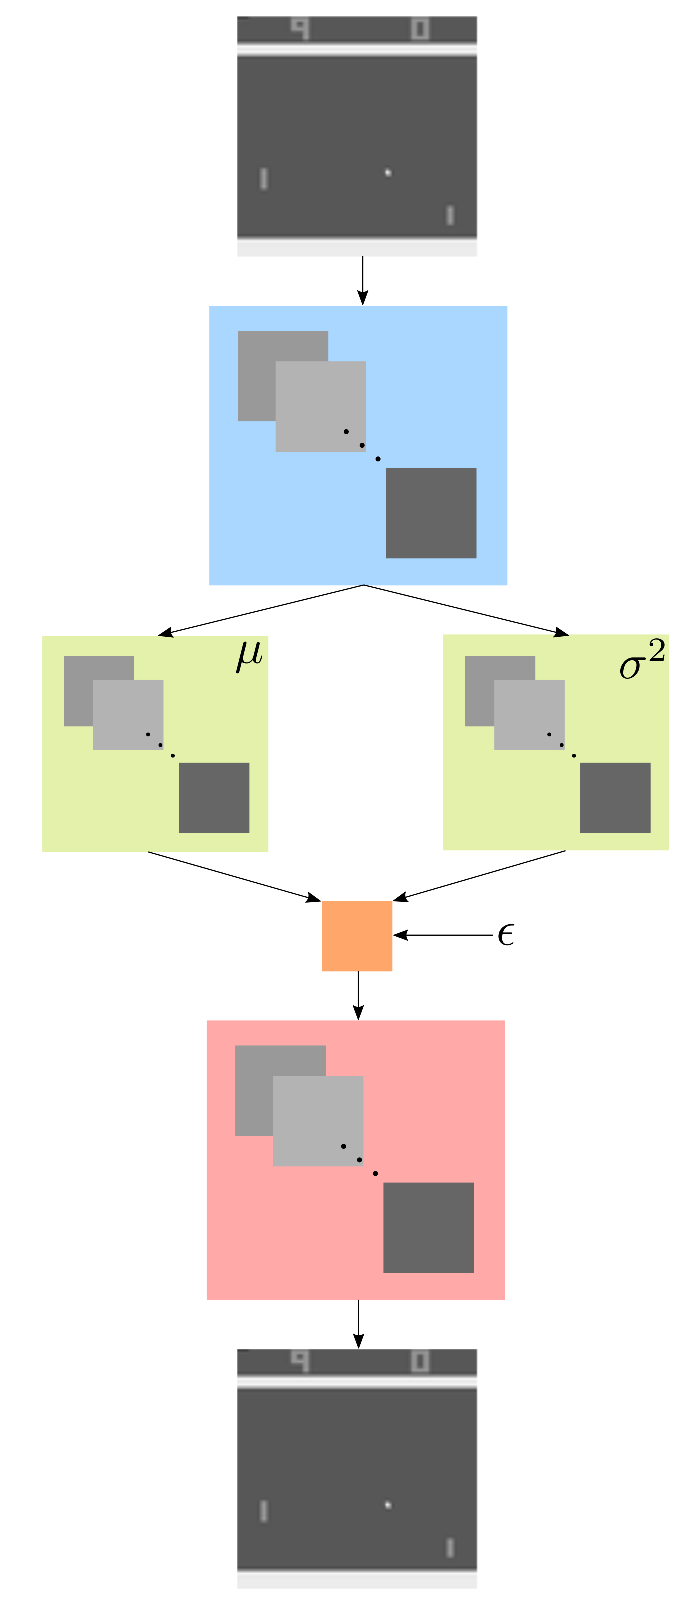
\includegraphics[scale=0.6]{methods/latent_image_architecture.eps}
\caption{The fully-convolutional single latent filter architecture. \textbf{Blue:} An arbitrary amount of convolutional layers. \textbf{Green:} The latent mean $\vec{\mu}$ and variance $\vec{\sigma}^2$, which are both single filters of shape $(1, m, n)$. \textbf{Orange:} A single latent filter of shape $(1, m, n)$ sampled component-wise from $\vec{\mu}$ and $\vec{\sigma}^2$. \textbf{Red:} The corresponding deconvolutional layers.}
\label{fig:latent_image_architecture}
\end{figure}

%
%
\subsection{Neuron-Level Redundancy Reduction}
As with all autoencoders, a reconstruction loss term must appear in the loss function as to learn the identity function, which ensures a meaningful lower-dimensional representation is learnt in the latent space. Hence we also include the reconstruction loss term 
\begin{align}
\mathbf{E}_{q_{\vec{\phi}}(\vec{z}|\vec{x})}\big[\log p_{\vec{\theta}}(\vec{x} | \vec{z}) \big]
\end{align}
in the final loss function for this architecture.

We also saw in $\beta$-VAE that the multiplicative factor on the KL loss term 
\begin{align}
-\beta D_{KL}(q_{\vec{\phi}}(\vec{z}|\vec{x}) || p_{\vec{\theta}}(\vec{z}))
\end{align}
varies the pressure of redundancy reduction on the latent space. As we seek to have non-zero activations in the latent space if and only if an object is present, it's in our interest to reduce the number of unnecessarily activated neurons. Therefore the application of a redundancy pressure term seems suitable, and is therefore included in the loss function. However, as we no longer have a one-dimensional latent space, we must decide on how this term will appropriately reduce redundancy in a two-dimensional latent space.

To reduce the redundancy in a two-dimensional latent space, we choose to flatten the $(1, m, n)$-dimensional single latent filter to an $m \times n$ vector $\vec{z}$, which is then matched to the prior $p(\vec{z})$, an isotropic Gaussian. We choose the prior to be $p(\vec{z}) = \mathcal{N}(\vec{0}, \vec{I})$ for convenience.\\

\begin{figure}[h!]
\centering
\captionsetup{justification=centering}
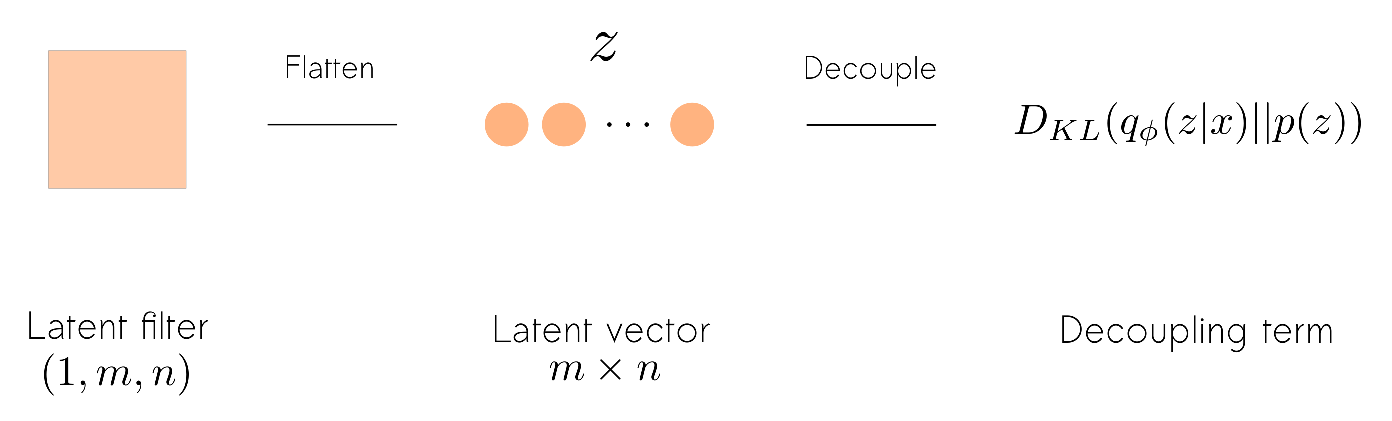
\includegraphics[scale=0.6]{methods/latent_image_flattening_latent_space.eps}
\label{fig:latent_image_flattening_latent_space}
\end{figure}

By reducing the two-dimensional latent space to one dimension, we arrive at the same loss function as in the $\beta$-VAE case:
\begin{align}
\mathcal{L}(\vec{\theta}, \vec{\phi}; \vec{x}) = -\beta D_{KL}(q_{\vec{\phi}}(\vec{z}|\vec{x}) || p_{\vec{\theta}}(\vec{z})) + \mathbf{E}_{q_{\vec{\phi}}(\vec{z}|\vec{x})}\big[\log p_{\vec{\theta}}(\vec{x} | \vec{z}) \big]
\end{align}


%
%
%
%
%
\section{Multiple Latent Filters}

Although it's conceivable that a single latent filter could represent types and locations of objects in the scene, it seems unlikely to do so. It's well known that filters may learn a set of weights to recognise information-rich features in the scene, like edges or corners. Perhaps this property could be leveraged by using multiple filters in the latent space, where any given latent filter is not responsible for representing multiple types of objects, but one specific object.

By the same reasoning for the single latent filter architecture, we keep the reconstruction loss 
\begin{align}
\mathbf{E}_{q_{\vec{\phi}}(\vec{z}|\vec{x})}\big[\log p_{\vec{\theta}}(\vec{x} | \vec{z}) \big]
\end{align}
to learn a meaningful low-dimensional representation in the latent space. However, we propose three techniques of redundancy reduction in the latent space to achieve our desiderata:
\begin{itemize}
\item Neuron-level redundancy reduction
\item Na\"{i}ve filter-level redundancy reduction
\item Weighted filter-level redundancy reduction
\end{itemize}

%
%
\subsection{Architecture}
The architecture is the same as the fully-convolutional single lantent filter architecture, but with strictly more than one filter in the latent space. The convolutional mean $\vec{\mu}$ and variance $\vec{\sigma}^2$, both of shape $(k, m, n)$, are sampled using the reparameterisation trick
\begin{align}
\vec{z} = g_{\vec{\phi}}(\vec{x}, \vec{\epsilon}) = \vec{\mu} + \vec{\sigma} \odot \vec{\epsilon} \quad\quad\quad \vec{\epsilon} \sim \mathcal{N}(\vec{0}, \vec{I})
\tag{\ref{eq:reparameterisation_trick}}
\end{align}
so we may use backpropagation. The corresponding deconvolutional layers are applied to reconstruct the original image.\\

\begin{figure}[h!]
\centering
\captionsetup{justification=centering}
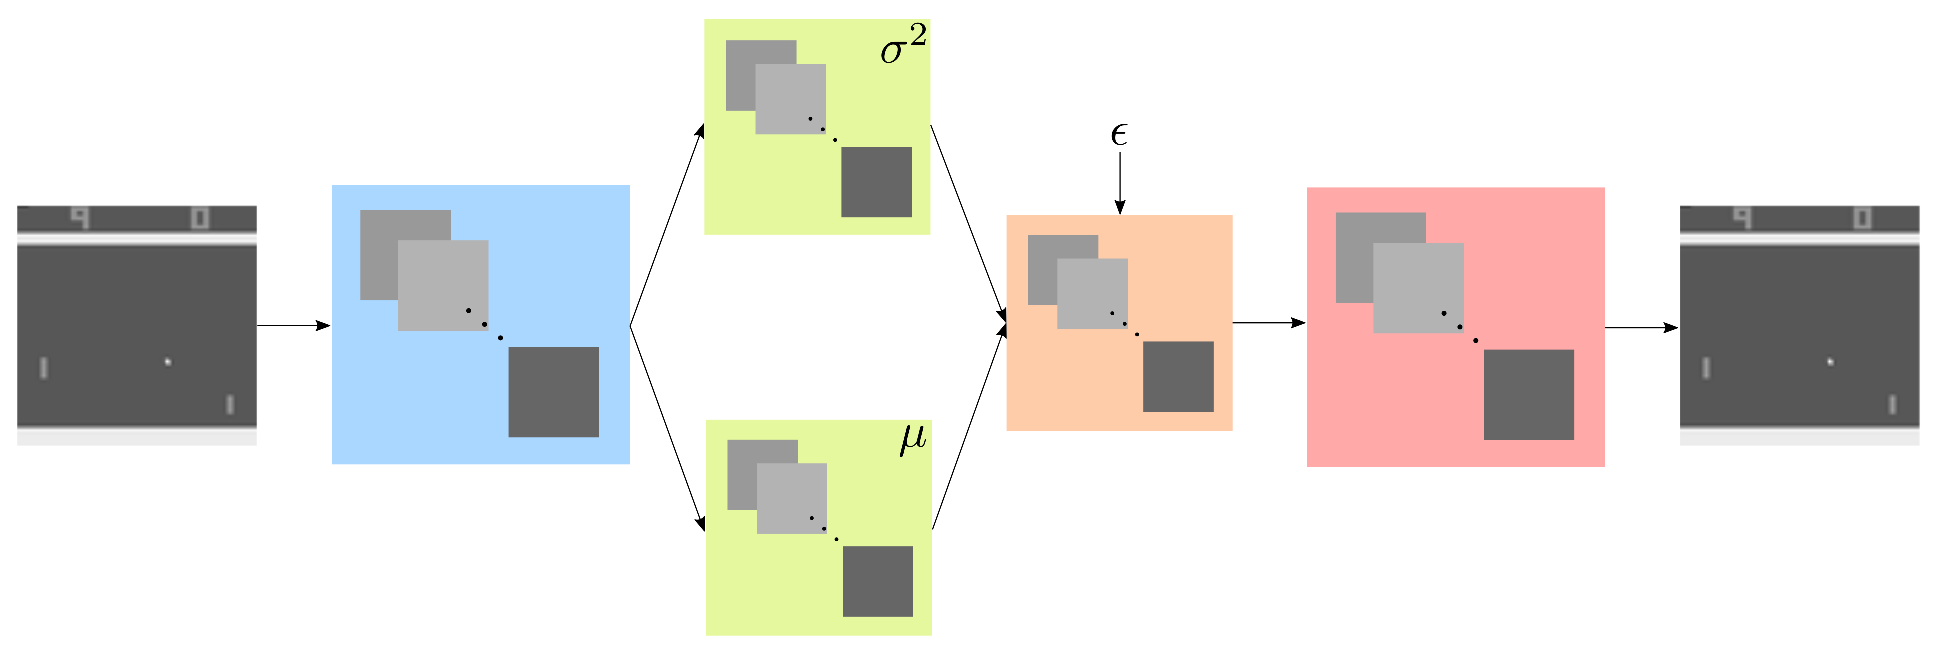
\includegraphics[scale=0.55]{methods/decoupling_indiscriminately_horizontal.eps}
\caption{The fully-convolutional multiple latent filter architecture. \textbf{Blue:} Unchanged. \textbf{Green:} The latent mean $\vec{\mu}$ and variance $\vec{\sigma}^2$, which are both single filters of shape $(k, m, n)$. \textbf{Orange:} A single latent filter of shape $(k, m, n)$ sampled component-wise from $\vec{\mu}$ and $\vec{\sigma}^2$. \textbf{Red:} Unchanged.}
\label{fig:decoupling_indiscriminately_horizontal}
\end{figure}

%
%
\subsection{Neuron-Level Redundancy Reduction}
To reduce the redundancy of activated neurons across the whole $(k, m, n)$-dimensional latent space, so that neurons are only activated when necessary, we apply neuron-level redundancy reduction. The latent filter of shape $(k, m, n)$ is flattened to a $k \times m \times n$ vector $\vec{z}$, which is then pressured to match the prior $p(\vec{z}) = \mathcal{N}(\vec{0}, \vec{I})$.\\

\begin{figure}[h!]
\centering
\captionsetup{justification=centering}
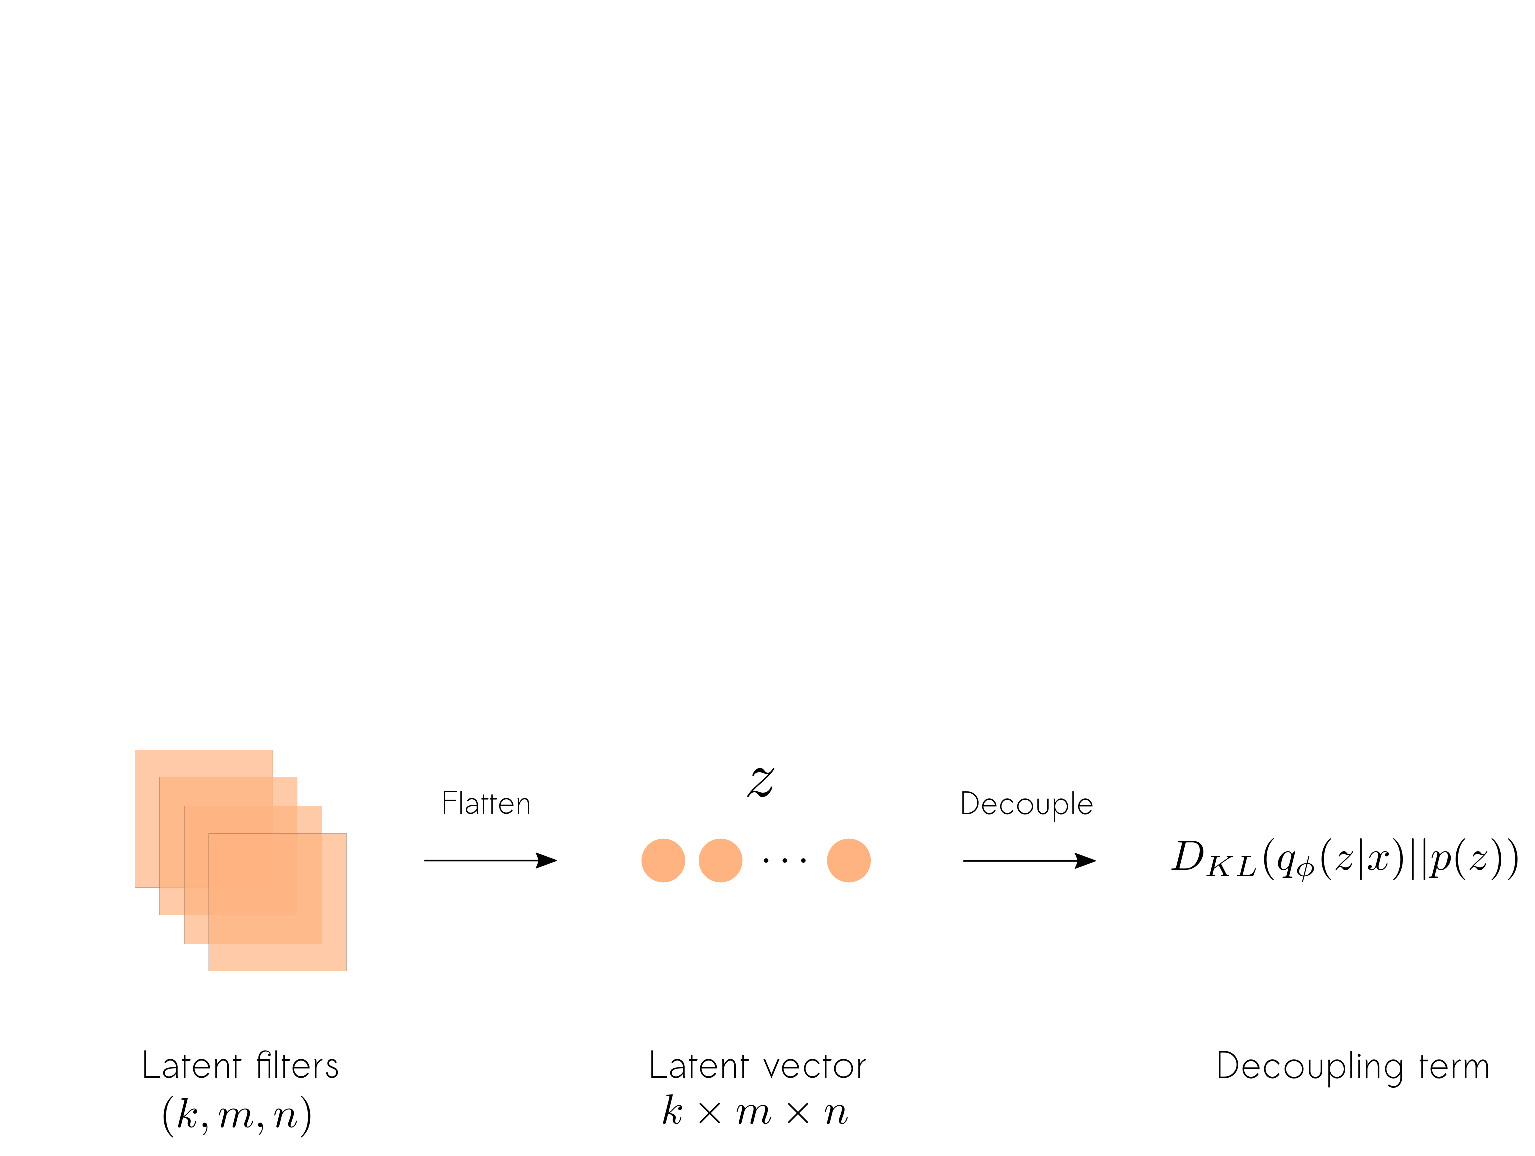
\includegraphics[scale=0.6]{methods/decoupling_indiscriminately_flattening_latent_space.eps}
\label{fig:decoupling_indiscriminately_flattening_latent_space}
\end{figure}

The loss function is therefore written as 
\begin{align}
\mathcal{L}(\vec{\theta}, \vec{\phi}; \vec{x}) = -\beta D_{KL}(q_{\vec{\phi}}(\vec{z}|\vec{x}) || p_{\vec{\theta}}(\vec{z})) + \mathbf{E}_{q_{\vec{\phi}}(\vec{z}|\vec{x})}\big[\log p_{\vec{\theta}}(\vec{x} | \vec{z}) \big]
\end{align}
where $\vec{z} \in \mathbb{R}^{k \times m \times n}$ is the flattened $(k, m, n)$-dimensional latent space.


%
%
\subsection{Na{\"i}ve Filter-Level Redundancy Reduction}

$\beta$-VAE sought to factorise the latent space into independent and dependent generative factors of the scene, in effect ``disentangling" the latent space. By similar reasoning, we'd like the activation of filters to clearly correspond to independent object types, with no two filters active for the same object. Hence we seek a factorisation over the activity of latent filters with no redundancy.

To achieve this, the $k$ filters of the $(k, m, n)$-dimensional latent space are averaged across their activations and stored in a vector $\vec{z}$. We then pressure the vector $\vec{z}$ to match the prior $p(\vec{z}) = \mathcal{N}(\vec{0}, \vec{I})$.\\

\begin{figure}[H]
\centering
\captionsetup{justification=centering}
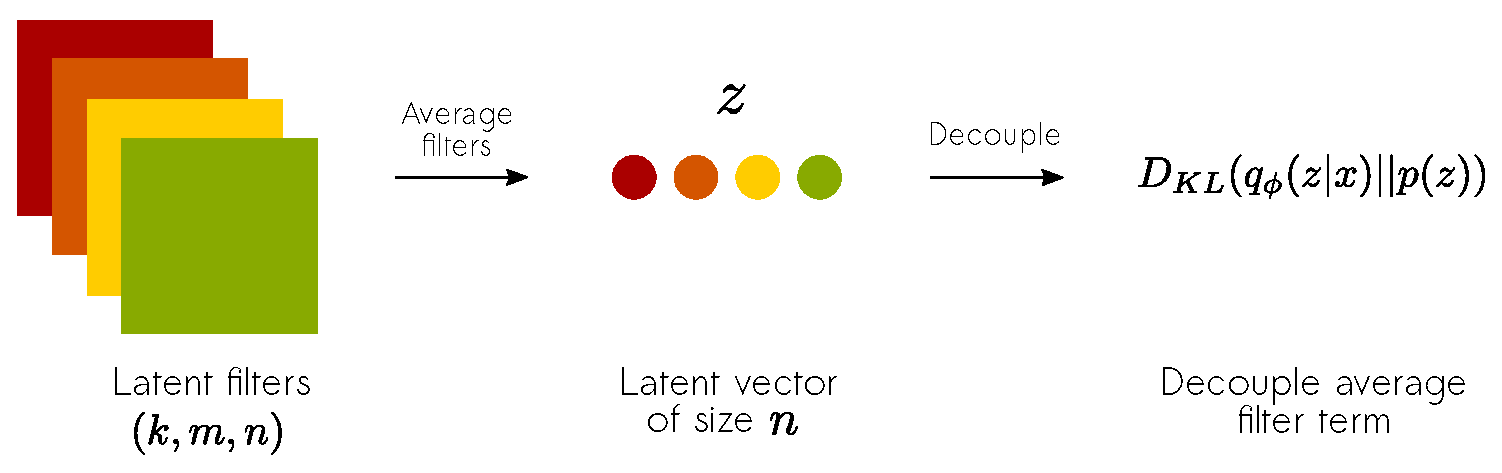
\includegraphics[scale=0.6]{methods/decoupling_averages_latent_space.eps}
\label{fig:decoupling_averages_latent_space}
\end{figure}

The loss function is therefore written as 
\begin{align}
\mathcal{L}_{NF}(\vec{\theta}, \vec{\phi}; \vec{x}) = -\beta D_{KL}(q_{\vec{\phi}}(\vec{z}|\vec{x}) || p_{\vec{\theta}}(\vec{z})) + \mathbf{E}_{q_{\vec{\phi}}(\vec{z}|\vec{x})}\big[\log p_{\vec{\theta}}(\vec{x} | \vec{z}) \big]
\end{align}
where $\vec{z} \in \mathbb{R}^{k}$ is the vector of averaged activations for each latent filter.


%
%
\subsection{Weighted Filter-Level Redundancy Reduction}
It's a subtle but necessary point that we should be careful to evaluate loss terms in a comparable way. For example, taking the sum of one and comparing it to the average of another (which is always less than the sum) serves to bias the loss function. This leads to the possibility that the average filter activation KL loss term in the naive filter-level redundancy technique is significantly under-represented when taking the sum reconstruction loss. (For simplicity, assume that we will take the sum reconstruction loss from here on.)

When evaluating the average filter activations, we get a single floating point number for $m \times n$ pixels, where $m$ and $n$ are the width and height of the latent filter respectively. Hence, when calculating the KL loss term, we may multiply by $m \times n$ so that the KL loss and reconstruction loss are of comparable size.\\

\begin{figure}[H]
\centering
\captionsetup{justification=centering}
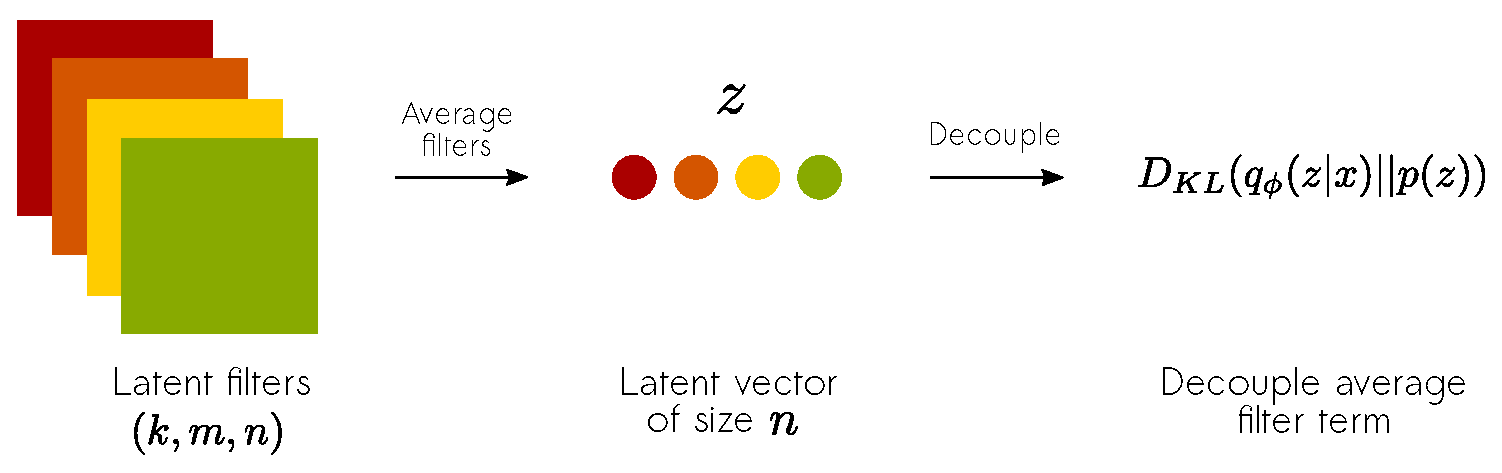
\includegraphics[scale=0.6]{methods/decoupling_averages_latent_space.eps}
\caption{Caption.}
\label{fig:decoupling_averages_latent_space}
\end{figure}

The loss function is therefore written as 
\begin{align}
\mathcal{L}_{WF}(\vec{\theta}, \vec{\phi}; \vec{x}) = -mn\beta D_{KL}(q_{\vec{\phi}}(\vec{z}|\vec{x}) || p_{\vec{\theta}}(\vec{z})) + \mathbf{E}_{q_{\vec{\phi}}(\vec{z}|\vec{x})}\big[\log p_{\vec{\theta}}(\vec{x} | \vec{z}) \big]
\end{align}
where $\vec{z} \in \mathbb{R}^{k}$ is the vector of averaged activations for each latent filter, and $m$ and $n$ are the width and height of the latent filters respectively.



%
%
%
%
%
\section{Separating Colour Spaces}

As the task of unsupervised object recognition in fully-convolutional variational autoencoders is an open problem, it's reasonable to start by solving easy recognition tasks. Since sprites in Atari games are of different colours, we can use these colour channels to make the separation of objects easier. An example for a frame of Space Invaders is shown in Figure (\ref{fig:separating_colour_spaces}). Since this technique is independent of architecture, it applies to all mentioned in the chapter.

%\begin{figure}[h!]
%\centering
%\captionsetup{justification=centering}
%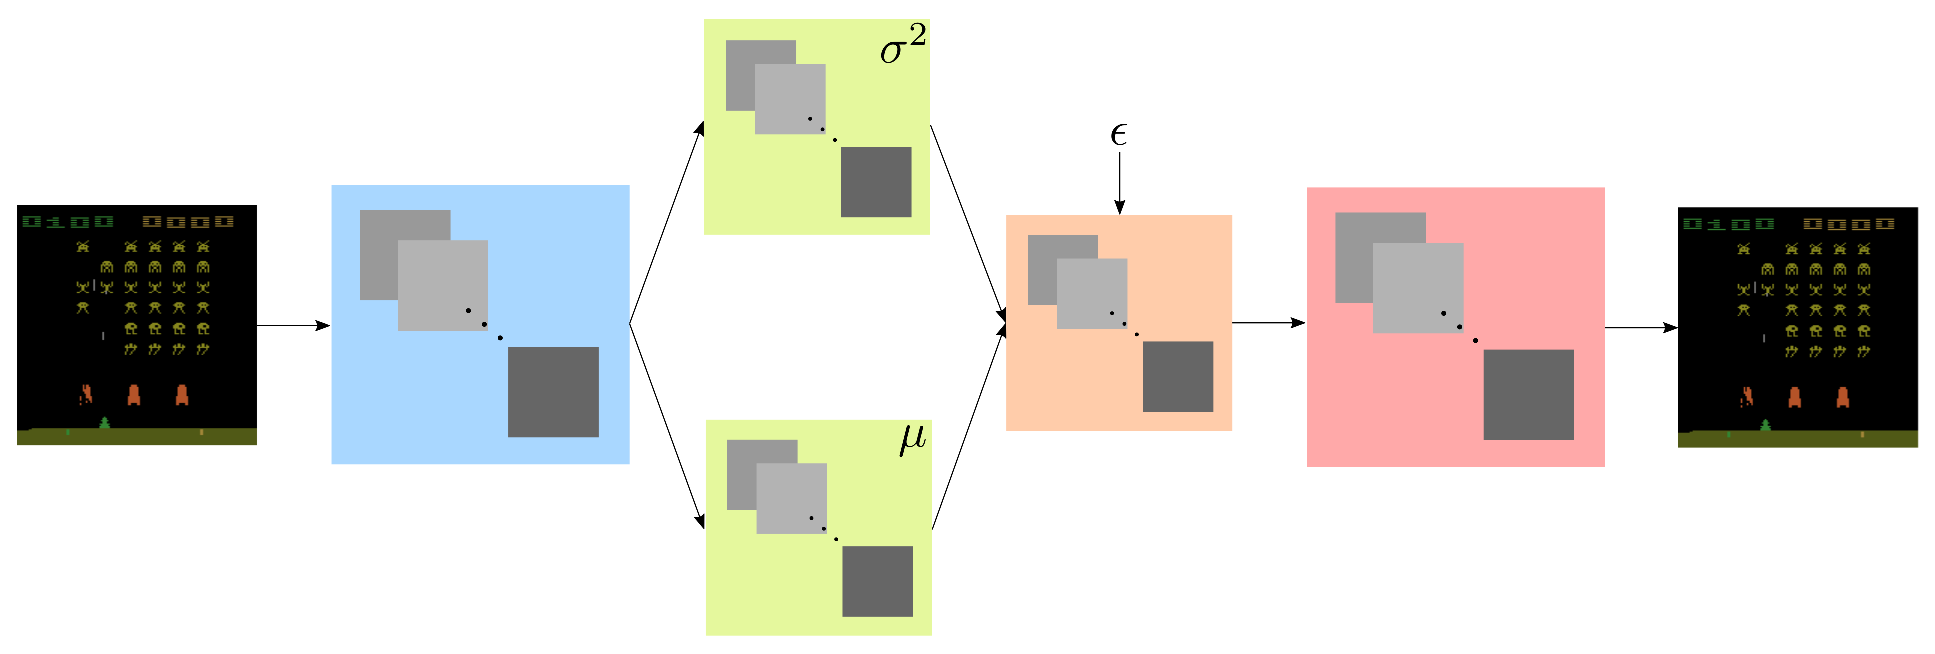
\includegraphics[scale=0.55]{methods/separating_colour_spaces_architecture.eps}
%\caption{Caption.}
%\label{fig:separating_colour_spaces_architecture}
%\end{figure}

\begin{figure*}[h!]
\centering
\captionsetup{justification=centering}
\begin{multicols}{4}
    \includegraphics[scale=0.7]{figures/methods/separating_colour_spaces_original.png}
    \caption{Original}\par
    \includegraphics[scale=0.7]{figures/methods/separating_colour_spaces_r.png}
    \caption{Red}\par
    \includegraphics[scale=0.7]{figures/methods/separating_colour_spaces_g.png}
    \caption{Green}\par
    \includegraphics[scale=0.7]{figures/methods/separating_colour_spaces_b.png}
    \caption{Blue}
\end{multicols}
\caption{A comparison of a $210 \times 160$ RGB frame from Space Invaders and its red, green and blue channels. The bullet is clearly separated from other sprites in the blue channel. The red and green channels separate collections of sprites. The red channel excludes the gunship and players score, while the green partially excludes the barriers.}
\label{fig:separating_colour_spaces}
\end{figure*}


One obvious limitation of this method is that the number of sprites separated is limited by the number of colour channels.



%
%
%
%
%
\section{Winner Takes All}

\begin{itemize}
\item As mentioned, it seems likely that objects may be classified by which latent filter has a high activation in its position
\item Assuming the latent space takes this structure, we would expect no more than one filter to be activated in any given position.
\item In other words, objects must have distinct types: a sprite cannot be a gunship and a number at the same time.
\item This leads to the Winner Takes All method, where we apply a position-wise pressure to the latent space so that no more than one filter has a high activation in any given position.
\item Naturally this applies to fully-convolutional multiple latent filter architectures.
\end{itemize}


\begin{figure*}[h!]
\centering
\captionsetup{justification=centering}
\begin{multicols}{2}
    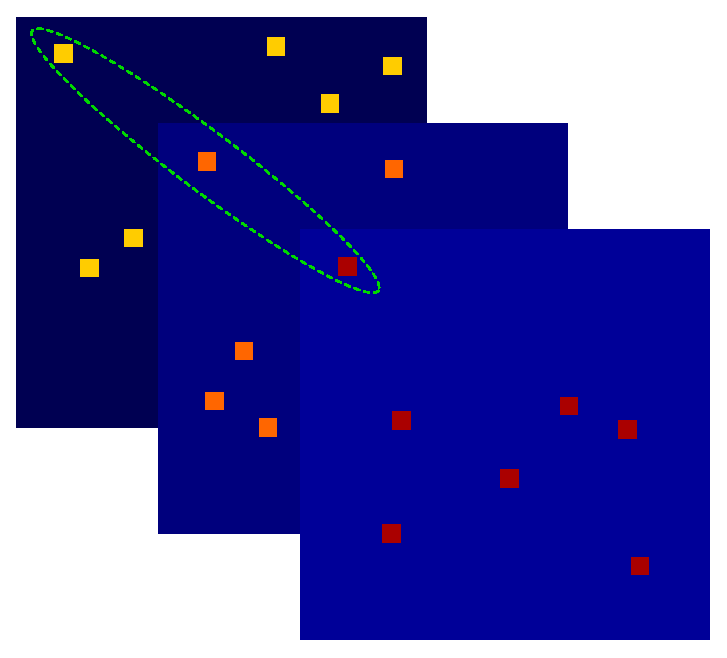
\includegraphics[scale=0.4]{figures/methods/winner_takes_all_object_on_every_filter.eps}
    \caption{Multiple types of objects recognised in same position.}
    \includegraphics[scale=0.4]{figures/methods/winner_takes_all_object_on_one_filter.eps}
    \caption{At most one object recognised in a given position.}
\end{multicols}
\caption{Caption.}
\label{fig:winner_takes_all_activations_on_layers}
\end{figure*}


\subsection{Derivation}

We wish to include a term in our loss function that ensures no more than one filter has a high activation in any given position.

Consider a convolutional latent space $\vec{z}$ of shape $(k, m, n)$. Let $\vec{z}^{i,j} \in \mathbb{R}^k$ be the vector storing the activations over the $k$ filters at position $(i, j)$. Naturally, we also let $q_{\vec{\phi}}^{i, j}(\vec{z} | \vec{x})$ represent the probabilistic encoder for $\vec{z}^{i,j}\in \mathbb{R}^k$. By matching the probabilistic encoder to an isotropic Gaussian we may reduce the redundancy, as argued previously. We choose to include the following term in our loss function:

\begin{align}
\sum_{i=1}^m \sum_{j=1}^n D_{KL}(q_{\vec{\phi}}^{i, j}(\vec{z} | \vec{x}) || p^{i,j}(\vec{z}))  \quad \textup{ where } \quad p^{i,j}(\vec{z}) = \mathcal{N}(\vec{0}, \vec{I})
\end{align}

As shown with $\beta$-VAE, the multiplicative $\beta$ controls the redundancy pressure. We will include this also and see if we observe a similar effect later.

\begin{figure}[h!]
\centering
\captionsetup{justification=centering}
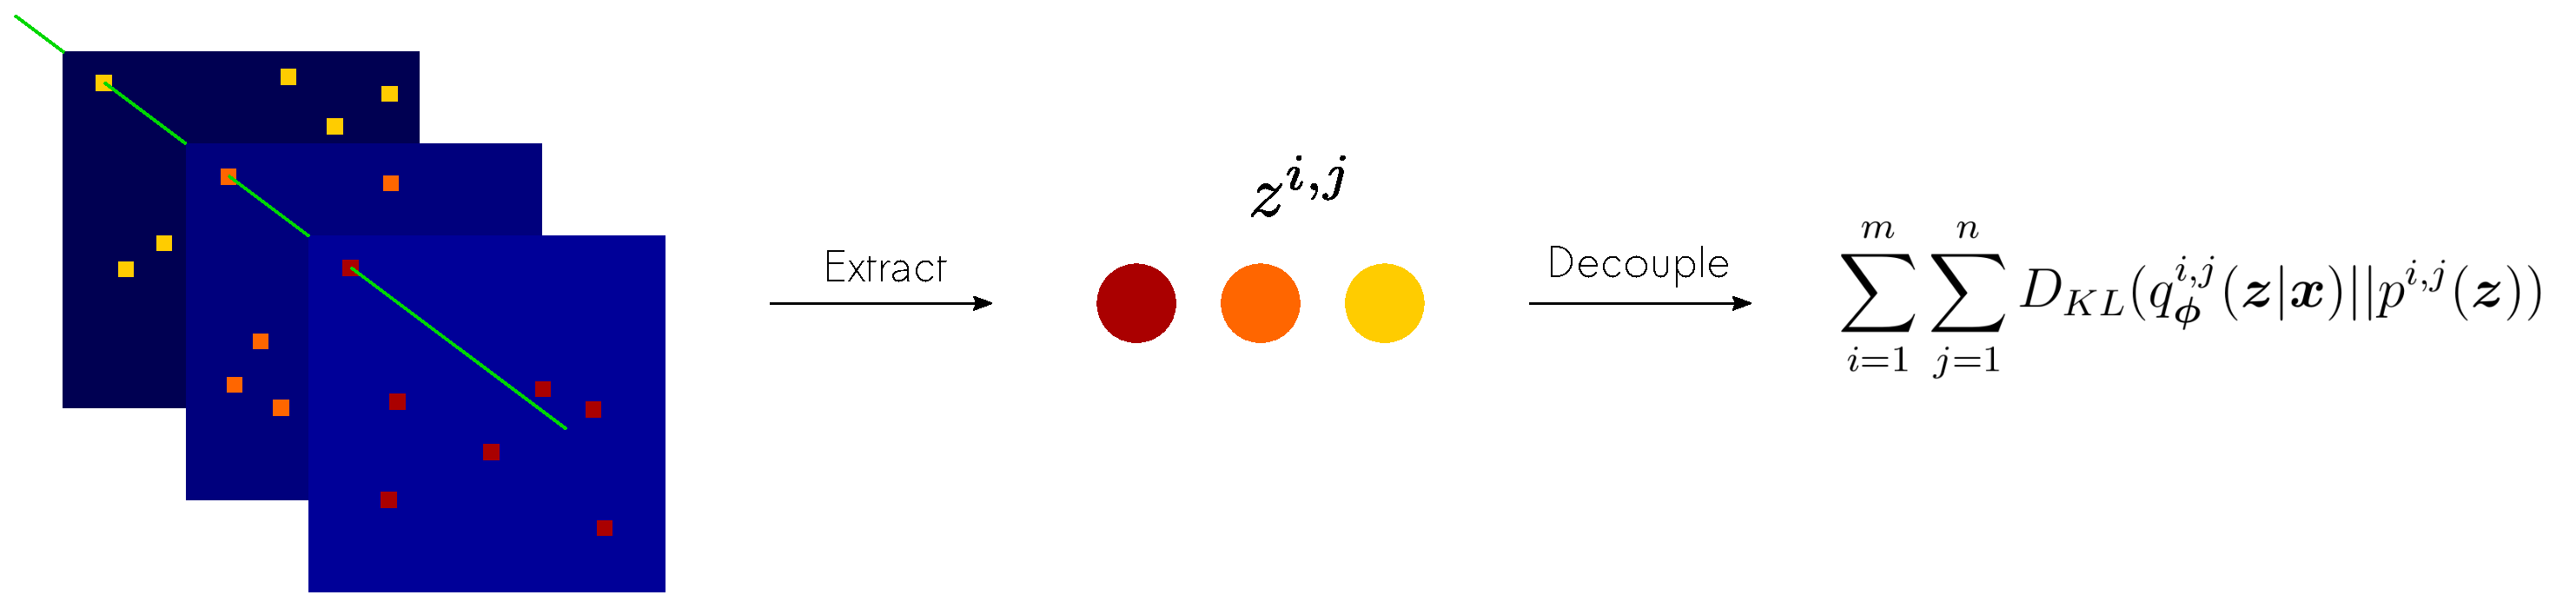
\includegraphics[scale=0.3]{methods/winner_takes_all_line_through_object_on_every_filter_flow_chart.eps}
\label{fig:winner_takes_all_line_through_object_on_every_filter}
\end{figure}

Therefore the final loss function is given as:

\begin{align}
\mathcal{L}_{WTA}(\vec{\theta}, \vec{\phi}; \vec{x}) = \mathbf{E}_{q_{\vec{\phi}}(\vec{z} | \vec{x})} \big[ \log p_{\vec{\theta}}(\vec{x} | \vec{z}) \big] - \beta \sum_{i=1}^m \sum_{j=1}^n D_{KL}(q_{\vec{\phi}}^{i, j}(\vec{z} | \vec{x}) || p^{i,j}(\vec{z})) 
\end{align}


%
%
%
%
%
\section{Orthogonal Convolutions}
\lipsum[2]
\subsection{Architecture}
TODO: Finish subsection
\begin{figure}[h!]
\centering
\captionsetup{justification=centering}
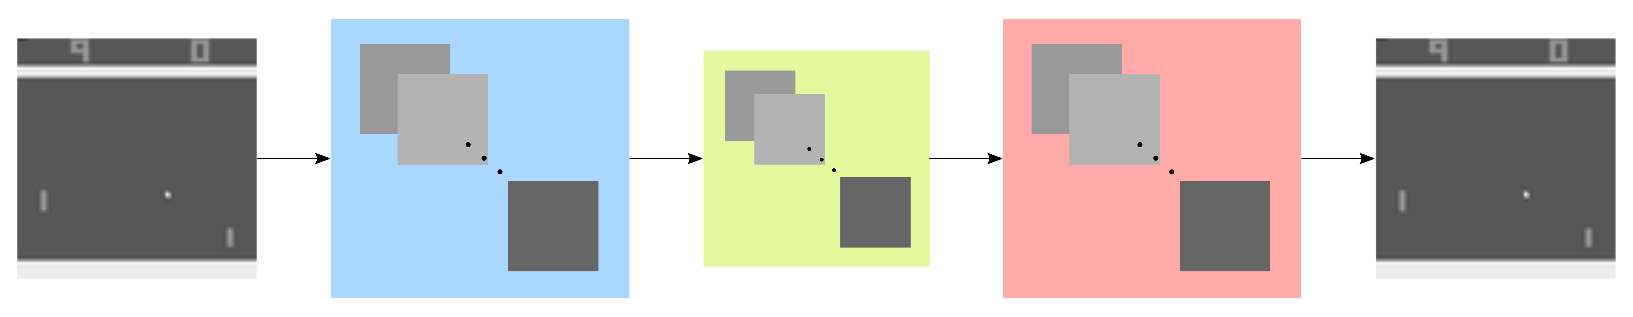
\includegraphics[scale=0.63]{methods/orthogonal_convolutions_archiecture.eps}
\caption{Caption.}
\label{fig:orthogonal_convolutions_archiecture}
\end{figure}

\subsection{Derivation}
TODO: Finish subsection